%!TEX root = ../../thesis.tex
\section{XHR Polling}

A simple method to check if there is new data on the client is to ask the server at certain intervals if it has new data for the client (``Polling''). The XMLHttpRequest\footnote{XMLHttpRequest is a technique that allows clients to send HTTP requests to servers. Although it has `XML' in its name, it actually supports arbitrary data formats. It is the most common way to request data in modern web clients.}(XHR) is the main data exchange technology used for this purpose. Sometimes, especially when it involves external APIs or legacy clients that do not support XHR, JSONP\footnote{JSONP is a technique to request data from servers by creating script-tags with a specific url. The server will then return JSON data encapsulated in a global callback function. Since there is no way to check if malicious code is being sent, this technique is considered insecure.} is used in its place but it is a limited, as well as insecure, way of handling client-server communication and is thus disregarded in this comparison.

\begin{figure}[htb]
  \centerline{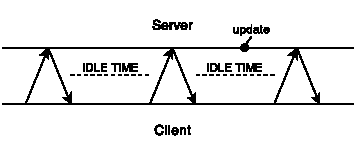
\includegraphics[width=0.8\linewidth]{images/Polling.pdf}}
  \caption[XHR Polling communication]{XHR Polling communication}
  \label{fig:polling}
\end{figure}

The simplest case for polling data from the server is shown in \reffigure{fig:polling}: the client periodically checks for new data on the server. If new data is received, it will be used to display the updated content. Afterwards, the client schedules a new request. The limitations of polling can easily be seen even from a simple example as presented in the figure above. The client will never receive updates in real-time and has a worst-case delay of IDLE-TIME. It should also be considered that there could be a large number of concurrently connected clients, all of whom request data at the same time interval. The server would need to handle request peaks in these intervals. Another weakness of polling is that it creates a traffic overhead by initiating too many unneeded requests.

One method to overcome some of these problems is to adapt the polling interval based on both the results of the first requests and the semantics of the requested information \cite{wanstrath2009pollinginterval}. If the requested information is based on an operation that needs a long time to finish, the polling interval could be adjusted to lengthen after each request. This would lead to fewer client requests and accordingly fewer request peaks. Yet still, this technique does not enable real-time updates.

\begin{figure}[htb]
  \centerline{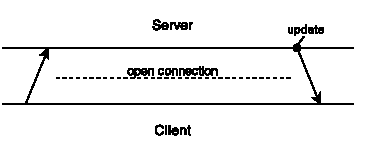
\includegraphics[width=0.8\linewidth]{images/Long_Polling.pdf}}
  \caption[XHR long polling communication]{XHR long polling communication}
  \label{fig:longpolling}
\end{figure}

An improvement to the standard polling mechanism is called long polling \cite[p. 276]{grigorik2013high}. Instead of asking for updates at a certain interval, clients connect to a server that will maintain an open connection until there is an update on the requested resource. The duration of the open connection from the client to the server is limited by a browser-specific timeout (circa 1-2min) but it is still much higher than the time between requests that is needed in classic polling. The typical connection flow of long-polling is shown in more detail in \reffigure{fig:longpolling}. Clients stay connected either until they time out or until the server responds with an update. Then they reconnect immediately after an update or a timeout.

This resolves some of the problems that occur with normal polling. Since clients timeout in different intervals, dependent on the browser vendor and the time of the update, servers will not have to handle request peaks. Through a reduction in the number of requests there is a significant decrease in traffic load on both sites, creating a much more efficient connection. Finally, updates occur in near real-time. The have a worst delay time of the amount time it takes to reconnect to the server.